\newpage
\section{Integration in EZyRB}
\label{sec:integration}
\texttt{EZyRB} is an open-source python package for data-driven model order reduction.
\texttt{EZyRB} provides three algorithms to compute the POD:
\begin{enumerate}
	\item Singular value decomposition from NumPy
	\item A randomized SVD, implemented using NumPy
	\item Solving the eigenvalue problem of the correlation matrix, implemented using NumPy
\end{enumerate}
NumPy provides fundamental linear algebra functions to python.
The implemented POD algorithms are only using NumPy and cannot make use of a cluster with several nodes.

Python provides the possibility to write modules in C/C++. We wrote such a module and included the hybrid POD implementation. The source code of this module can be found in the appendix \ref{list:cPODpython} and on GitHub \url{https://github.com/Flousen/EZyRB}.

The MPI functionality is provided to \texttt{EZyRB} by the
python package MPI4PY (MPI for Python)
\cite{DALCIN20111124}\cite{DALCIN20051108}\cite{DALCIN2008655}.
This package also provides c headerfiles that allow us to pass the MPI communicators from python to the C module.
This makes the integration of the hybrid implementation into \texttt{EZyRB} very simple.







\newpage
\subsection{Problem Heat Conduction}
\label{sec:HeatConduction}
In this Section, we describe a simple parametric PDE. The example is taken from \cite[Section 2.3.1]{HRSbook}.

We consider a simple heat conduction problem with two parameters on a two-dimensional domain.
The domain is defined as a rectangle. In the middle of the rectangle, there is a circle.
This circle has a different conductivity than the rest of the rectangle.
We call the circle $\Omega_1$ and the rest of the rectangle $\Omega_2$ (see Figure \ref{fig:scetchHeat}).
The conductivity of $\Omega_1$ is defined by the first parameter $\kappa = \mu_{0}$.
The conductivity of $\Omega_2$ is set to one $\kappa = 1$.
The boundary of the domain $\partial \Omega$ is split in three parts.
The two side edges of the rectangle $\Gamma_{side}$, the top edge $\Gamma_{top}$, and the bottom edge $\Gamma_{base}$.

The scalar field variable $u(\mu)$ is the temperature that satisfies Poisson’s equation in $\Omega$.
With the boundary conditions:
\begin{itemize}
	\item Homogeneous Neumann conditions on the side boundaries $\Gamma_{side}$. With this condition we have no heat  flux on the side edges.
	This modeling a insulation of the sides.
	\item Homogeneous Dirichlet condition on the top edge boundary $\Gamma_{top}$. This is modeling a constant temperature of zero on the edge.
	\item Parametrized Neumann conditions on the bottom edge boundary $\Gamma_{base}$. The heat flux over the bottom edge is given by the second parameter $\mu_1$.
\end{itemize}

\begin{figure}[H]
	\centering
	\scalebox{0.8}{
	\tikzset{
	main/.style={black, line width=0.4mm, opacity=1},
	second/.style={gray, opacity=5},
	arrow/.style={-latex, shorten >=1ex, shorten <=1ex, bend angle=45}
}
\begin{tikzpicture}
%% Grid


\node (rect) at (3,3) [draw,main,minimum width=6cm,minimum height=6cm,  fill=blue!30] {};
\draw (3,3) node[circle, main,minimum width=3cm,draw, fill=white] {};
\draw (3,3) node[circle, main,minimum width=3cm,draw, fill=red!60] {};

%\node (rect) at (3,3) [draw,main,minimum width=6cm,minimum height=6cm] {};
%\draw (3,3) node[circle, main,minimum width=3cm,draw, fill=white] {};
%\draw (3,3) node[circle, main,minimum width=3cm,draw] {};


\draw (1,5) node {$\Omega_{2}$};
\draw (2.5 , 3.5) node {$\Omega_{1}$};

\draw (3 , 2) node {$\kappa = \mu_0$};
\draw (2 , 1) node {$\kappa = 1$};

\draw [arrow, main]  ( 3 , 3 ) to ( 4.15 , 4.15 );
\draw (3.75 , 3.35) node {$ r_0 $};

% Rand		
\draw (3 , 6.5) node {$\Gamma_{top}$};
\draw (3 , -0.5) node {$\Gamma_{base}$};
\draw (-0.5 , 3) node {$\Gamma_{side}$};
\draw (6.5 , 3) node {$\Gamma_{side}$};


\end{tikzpicture}
	}
	\caption[Sketch domain]{Sketch of the domain with different thermal conductivity coefficients.}
	\label{fig:scetchHeat}
\end{figure}

There are two parameters in the problem. The conductivity $\mu_0$ of $\Omega_1$ and the temperature of the base edge $\mu_1$.\\
The parameter space is defined by $\mathbb{P} = [\mu_{0}^{min},\mu_{0}^{max}] \times [\mu_{1}^{min},\mu_{1}^{max}]$. The parameter vector ist defined by $\mu = (\mu_0, \mu_1)^T \in \mathbb{P}$.

The strong formulation of the para\-meterized problem is given by:\\
for a given parameter $\mu \in \mathbb{P}$, find $u(x,\mu)$ such that
\begin{align}
\begin{cases}
- \nabla \cdot (\kappa(x,\mu)\nabla u(x,\mu)) = 0 	& \text{in } \Omega 		\\
u(x,\mu) = 0 										& \text{on } \Gamma_{top} 	\\
\kappa(\mu)\nabla u(x,\mu)\cdot \mathbf{n} = 0 		& \text{on } \Gamma_{side} 	\\
\kappa(\mu)\nabla u(x,\mu)\cdot \mathbf{n} = \mu_1 	& \text{on } \Gamma_{base} 	\\
\end{cases}
\end{align}


where 
\begin{itemize}
	\item $\mathbf{n}$ denotes the outer normal to the boundaries $\Gamma_{side}$ and $\Gamma_{base}$,
	\item the conductivity $\kappa(x,\mu)$ is defined as follows:
	\begin{align}
		\kappa(x,\mu) =
		\begin{cases}
		\mu_0, & x \in \Omega_1\\
		1, & x \in \Omega_2
		\end{cases}		
	\end{align}
\end{itemize}

The functional space is defined as $\mathbb{X} = \left\{ v \in H^1(\Omega): v|_{\Gamma_{top}} = 0 \right\}$.
The weak formulation is obtained by multiplying a test function $v\in \mathbb{X}$ on the function and then integrate over the domain $\Omega$
\begin{align*}
	-&\nabla \cdot (\kappa(x,\mu)\nabla u(x,\mu)) v(x) = 0\\
	-\int_{\Omega} &\nabla \cdot (\kappa(x,\mu)\nabla u(x,\mu)) v(x) d\boldsymbol{x} = 0
\end{align*}
We integrate by part
\begin{align*}
	&\int_{\Gamma_{top}} \kappa(x,\mu)\nabla u(x,\mu) v(x) d\boldsymbol{x}
	+
	\int_{\Gamma_{side}} \kappa(x,\mu)\nabla u(x,\mu) v(x) d\boldsymbol{x}\\
	+
	&\int_{\Gamma_{base}} \kappa(x,\mu)\nabla u(x,\mu) v(x) d\boldsymbol{x}
	+
	\int_{\Omega} \kappa(x,\mu)\nabla u(x,\mu) \nabla v(x) d\boldsymbol{x} = 0.
\end{align*}
The boundary integral over $\Gamma_{top}$ disappears because we choose the test functions $v \in \mathbb{X}$, all functions in $\mathbb{X}$ are zero on $v|_{\Gamma_{top}} = 0$.
The boundary integral over $\Gamma_{side}$ disappears because of the Neumann boundery condition $\kappa(\mu)\nabla u(x,\mu)\cdot \mathbf{n} = 0$.
The boundary integral over $\Gamma_{base}$ can be written as $\mu_1 \int_{\Gamma_{base}} v \text{d}s$ on the right hand side.

The corresponding weak formulation reads:
for a given parameter $\mu\in\mathbb{P}$,
\begin{align*}
\text{find }u \in \mathbb{X} :\quad a\left(u,v;\mu\right) = f(v;\mu) \quad \forall v\in\mathbb{X}
\end{align*}
where
\begin{itemize}
	\item the parametrized bilinear form $a(\cdot, \cdot; \mu)$ is defined by:
	\begin{align*}
		a(u, v;\mu)
		&=\int_{\Omega} \kappa(\mu)\nabla u(x,\mu)\cdot \nabla v(x) \ d\boldsymbol{x} ,
	\end{align*}
	\item the affine decompositions are defined by:
	\begin{align*}
		a(u, v;\mu)
		&=\int_{\Omega} \kappa(\mu)\nabla  u(x,\mu)\cdot \nabla v(x) \ d\boldsymbol{x} \\
		&= \mu_0 \int_{\Omega_1} \nabla u(x,\mu)\cdot \nabla v(x) \ d\boldsymbol{x} 
		+ \int_{\Omega_2} \nabla u(x,\mu)\cdot \nabla v(x) \ d\boldsymbol{x} ,
	\end{align*}
	
	\item the parametrized linear form $f(v;\mu)$ is defined by:
	\begin{align*}
	f(v;\mu) &= \mu_1 \int_{\Gamma_{base}} v \text{d}s.
	\end{align*}

\end{itemize}

\newpage
\subsection{EZyRB benchmarks}
To show the functionality of our algorithm we used it on the data from \texttt{tutorial 1} from \texttt{EZyRB} \cite{demo18ezyrb}. In the example the snapshots of the corresponding parameters and the mesh informations are included. 
For that tutorial eight snapshot of the example described above in Section \ref{sec:HeatConduction} were created using \texttt{FEnics}.
The parameter space $\mathbb{P}$ was sampled, in a range $\mathbb{P} =  [0, 10] \times  [-1,1]$, with the following eight parameter combinations
\begin{align*}
\Xi_{train}=
\left\{
\begin{pmatrix} 0.5 \\ -0.2 \end{pmatrix},
\begin{pmatrix} 8.6 \\  0.1 \end{pmatrix},
\begin{pmatrix} 5.3 \\  0.8 \end{pmatrix},
\begin{pmatrix} 9.4 \\  0.1 \end{pmatrix},
\begin{pmatrix} 7.3 \\ -0.8 \end{pmatrix},
\begin{pmatrix} 0.2 \\  0.8 \end{pmatrix},
\begin{pmatrix} 3.5 \\ -0.5 \end{pmatrix},
\begin{pmatrix} 0.3 \\  0.6 \end{pmatrix}
\right\}.
\end{align*}
Figure \ref{fig:snaps} shows plots of the snapshots.
The plots show the mesh information and the heat distribution.
\begin{figure}[H]
	\centering
	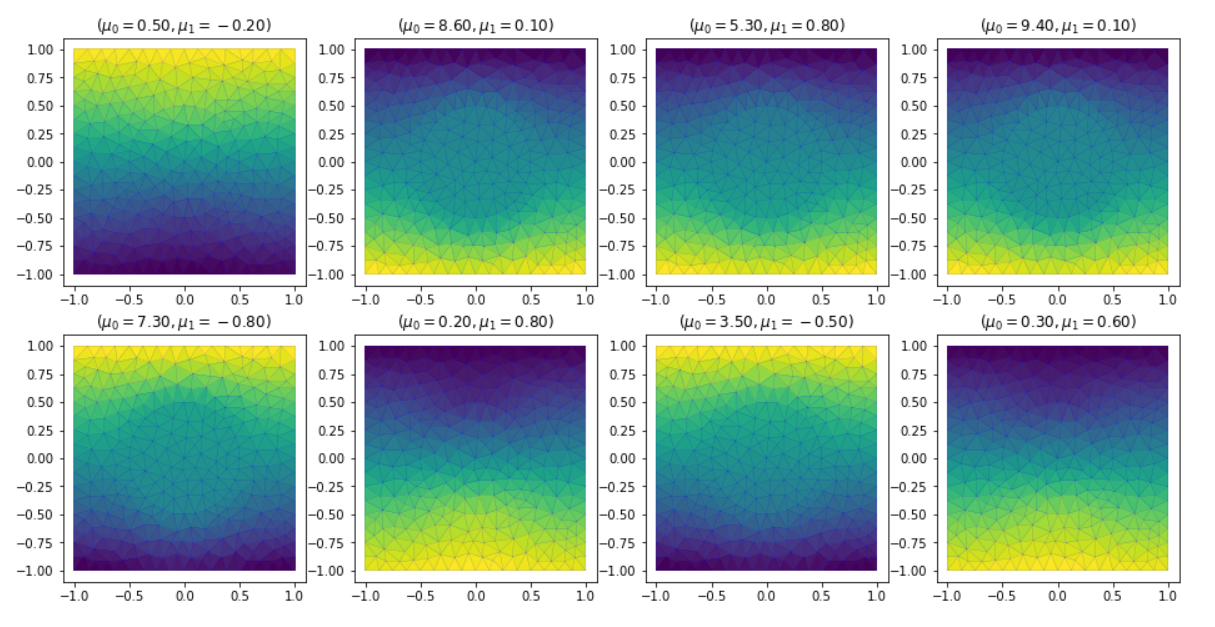
\includegraphics[width=\textwidth]{images/snapshots}
	\caption[Snapshots]{Heat distribution for the differen snapshots. }
	\label{fig:snaps}
\end{figure}

We created a reduced model from the snapshots using our algorithm.
In Figure \ref{fig:Singularvals} the value of the singular values respectively the square root of the eigenvalues is plotted.
We can see that the singular values shrink a lot between the first two modes. The following values are also shrinking but with a smaller magnitude than the first ones.

This behavior can be observed in practice. The first singular values have the biggest magnitude and decrease fast. The  modes with the singular values that fall no longer significantly can be truncated as discussed in Section \ref{sec:POD}. 

\begin{figure}[H]
	\centering
	% This file was created by matlab2tikz.
%
%The latest updates can be retrieved from
%  http://www.mathworks.com/matlabcentral/fileexchange/22022-matlab2tikz-matlab2tikz
%where you can also make suggestions and rate matlab2tikz.
%
\definecolor{mycolor1}{rgb}{0.00000,0.44700,0.74100}%
\definecolor{mycolor2}{rgb}{0.85000,0.32500,0.09800}%
\definecolor{mycolor3}{rgb}{0.92900,0.69400,0.12500}%
%
\begin{tikzpicture}

\begin{axis}[%
width=4.521in,
height=3.566in,
at={(0.758in,0.481in)},
scale only axis,
xmin=0.25,
xmax=8.25,
xlabel style={font=\color{white!15!black}},
xlabel={POD modes},
ymin=0,
ymax=950,
ylabel style={font=\color{white!15!black}},
ylabel={},
axis background/.style={fill=white},
axis x line*=bottom,
axis y line*=left,
legend style={at={(0.97,0.97)}, anchor=north east, legend cell align=left, align=left, draw=white!15!black}
]

\addplot [color=mycolor1, mark=+, mark options={solid, mycolor1, scale=2}]
table[row sep=crcr]{%
	1	874.5893 \\
	2	58.1832  \\
	3	48.2328  \\
	4	45.9105  \\
	5	35.5212  \\
	6	23.8663  \\
	7	20.6150  \\
	8	15.4926  \\
};
%\addlegendentry{Eigen values}

\end{axis}
\end{tikzpicture}%
	\caption[Singular values]{Singular values of the corresponding POD modes}
	\label{fig:Singularvals}
\end{figure}

For this simple example we didn't do the truncation.
Figure \ref{fig:reconstruct} shows a reconstucted solution with the parameter $ \bar{\mu} = (\bar{\mu}_1 , \bar{\mu}_2 )^T = ( 8 , 1 )^T $.
\begin{figure}[H]
	\centering
	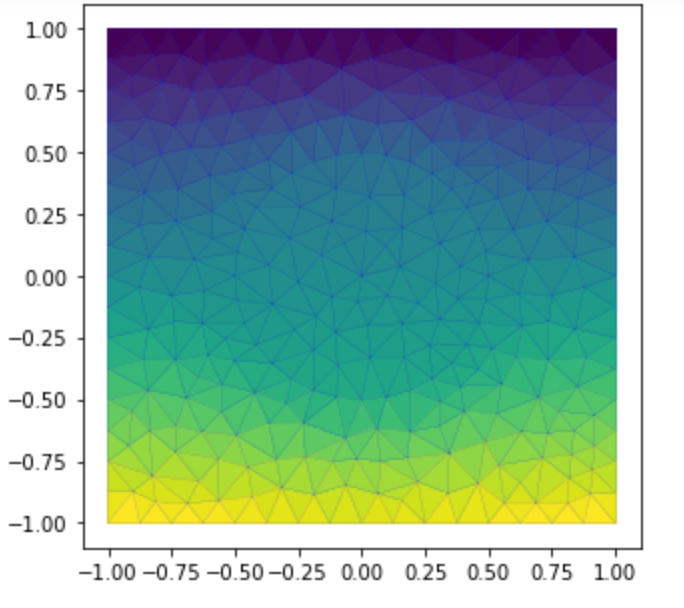
\includegraphics[width=0.38\textwidth]{images/reconstruct}
	\caption[Reduced Solution]{A solution computed with the reduced model created with \texttt{EZyRB}}
	\label{fig:reconstruct}
\end{figure}

\subsubsection{Benchmark}
With the data from tutorial 1 from \texttt{EZyRB} \cite{demo18ezyrb} we showed that the algorithm works properly, but it is not suitable to evaluate the performance.

To evaluate the performance we used a snapshot matrix with the same dimension as in Section \ref{sec:Benchmarks} and measured the time the POD class needs to compute the POD modes. This benchmark shows the performance we loose by using the python layer.

Due to issues with the cluster we had to do this benchmark on a different cluster. The new cluster has processors with 16 cores.
In Figure \ref{fig:ezybench} we can see that the measuring points increase in steps of 16 processors and not in steps of 10 like the benchmarks in Section \ref{sec:Benchmarks}.
We can still see that the implementation performed similar to the other benchmark in Figure \ref{fig:bench5} from Section \ref{sec:hybrid}.
\begin{figure}[H]
	\centering
	% This file was created by matlab2tikz.
%
%The latest updates can be retrieved from
%  http://www.mathworks.com/matlabcentral/fileexchange/22022-matlab2tikz-matlab2tikz
%where you can also make suggestions and rate matlab2tikz.
%
\definecolor{mycolor1}{rgb}{0.00000,0.44700,0.74100}%
\definecolor{mycolor2}{rgb}{0.85000,0.32500,0.09800}%
\definecolor{mycolor3}{rgb}{0.92900,0.69400,0.12500}%
%
\begin{tikzpicture}

\begin{axis}[%
width=4.521in,
height=3.566in,
at={(0.758in,0.481in)},
scale only axis,
xmin=0,
xmax=132,
xlabel style={font=\color{white!15!black}},
xlabel={Number of Processors},
ymin=0,
ymax=14.2,
ylabel style={font=\color{white!15!black}},
ylabel={Speed up},
axis background/.style={fill=white},
axis x line*=bottom,
axis y line*=left,
legend style={at={(0.03,0.97)}, anchor=north west, legend cell align=left, align=left, draw=white!15!black}
]

\addplot [color=mycolor3, mark=+, mark options={solid, mycolor3}]
table[row sep=crcr]{%
1     0.926193820542935\\
16    5.564527272810553\\
32    8.253695032798474\\
48    9.810377172379205\\
64    10.85966997160303\\
80    11.87933924922592\\
96    12.30403623120082\\
112   12.67579337348104\\
128   13.13623736917454\\
};
%\addlegendentry{EZyRB}




\end{axis}
\end{tikzpicture}%
	\caption[EZyRB Benchmark]{Benchmark integrated in the reduced order modeling framework \texttt{EZyRB}}
	\label{fig:ezybench}
\end{figure}


\newpage
\section{Conclusion}
We presented two algorithms to compute the POD in parallel.
A parallel algorithm using the singular value decomposition (SVD) and a parallel algorithm solving the eigenvalue problem of the correlation matrix (EVP).
Both algorithms performed good in case the snapshot matrix is already distributed to the different processors.
We saw that the EVP algorithm performs best, due to its limited number of operations.

For the case that the snapshot matrix is not distributed to the processors the algorithm got improved.
%We also tried to improve this algorithm for the case that the snapshot matrix is not yet distributed to the processors.
We proposed a hybrid implementation to overcome the number of communications.

Finally we  integrated the hybrid implementation into the reduced order modeling framework \texttt{EZyRB}.
We tested the new algorithm using \texttt{EZyRB} and also benchmarked the algorithm in the Python package.
With the parallel algorithm \texttt{EZyRB} can now make use af high perfomance cluster for the POD modes extraction.

In future works one could try to speed up the computation of the correlation matrix for the case that the snapshot matrix is not distributed.
Scattering the snapshot matrix to the processors is an expensive operation and slows down the overall POD computation a lot.
Instead of scattering the snapshot matrix to the processors, one could try to use Graphics Processing Units (GPU) for the computation of the correlation matrix.
GPUs are well suited these kine of operations.




